\documentclass{article}
\usepackage[implicantcolors]{karnaugh-map}
\usepackage{xstring}
\usepackage{geometry}[margin=1in]
\usepackage{hyperref}
\usepackage{xcolor}
\usepackage{keyval}
\usepackage{kvoptions}
\usepackage[table]{xcolor}
\definecolor{lightred}{HTML}{FFB6C1}
\definecolor{lightorange}{HTML}{FFDAB9}
\definecolor{lightyellow}{HTML}{FFFFE0}
\definecolor{lightgreen}{HTML}{BCF5BC}
\definecolor{lightblue}{HTML}{9FD8EF}
\definecolor{lightpurple}{HTML}{E6E6FA}
\hypersetup{
    colorlinks=true,
    linkcolor=black,
    filecolor=magenta,      
    urlcolor=cyan,
    pdfpagemode=FullScreen,
}
\urlstyle{same}
\begin{document}
\title{2E04: Design Project}
\author{sur21}
\date{December 13th, 2024}
\maketitle
\newpage
\tableofcontents
\newpage
\section{Analytical Solution}
\subsection{Student Number Binary Conversion}
My student number is 400507973. This will give binary conversion of:
\\
\begin{tabular}{|c|c|c|c|}
    \hline
    Digit & Current State ($Q_1Q_2Q_3Q_4$) & Counters ($C_1C_2$) & Don't Care\\
    \hline
    4 & 0100 & 00 & * \\
    \hline
    0 & 0000 & 01 & -\\
    \hline
    0 & 0000 & 10 & -\\
    \hline
    5 & 0101 & 11 & * \\
    \hline
    0 & 0000 & 00 & -\\
    \hline
    7 & 0111 & 01 & -\\
    \hline
    9 & 1001 & 10 & * \\
    \hline
    7 & 0111 & 11 & -\\
    \hline
    3 & 0011 & 00 & * \\
    \hline
\end{tabular}
\vspace{0.5\baselineskip}
\\
For the don't care unique digits, its counter states can be chosen to be anything. For the repeating digits, 0 and 7, its counter states can be arranged in a way such that
the counters form a loop a simple loop, making the logic easier to implement and K-Map.
\subsection{Excitation Table}
\begin{tabular}{|c|>{\columncolor{lightred}}c|>{\columncolor{lightorange}}c|>{\columncolor{lightyellow}}c|>{\columncolor{lightgreen}}c|>{\columncolor{lightblue}}c|>{\columncolor{lightpurple}}c|>{\columncolor{lightred}}c|>{\columncolor{lightred}}c|>{\columncolor{lightorange}}c|>{\columncolor{lightorange}}c|>{\columncolor{lightyellow}}c|>{\columncolor{lightyellow}}c|>{\columncolor{lightgreen}}c|>{\columncolor{lightgreen}}c|>{\columncolor{lightblue}}c|>{\columncolor{lightblue}}c|>{\columncolor{lightpurple}}c|>{\columncolor{lightpurple}}c|}
    \hline
    \# & $Q_1$ & $Q_2$ & $Q_3$ & $Q_4$ & $C_1$ & $C_2$ & $J1$ & $!K1$ &  $J2$ & $!K2$ & $J3$ & $!K3$ & $J4$ & $!K4$ &  $J_{C_1}$ & $!K_{C_1}$ & $J_{C_2}$ & $!K_{C_2}$ \\
    \hline
    4 & 0 & 1 & 0 & 0 & 0 & 0 & 0 & X & X & 0 & 0 & X & 0 & X & 0 & X & 1 & X \\
    \hline
    0 & 0 & 0 & 0 & 0 & 0 & 1 & 0 & X & 0 & X & 0 & X & 0 & X & 1 & X & X & 0 \\
    \hline
    0 & 0 & 0 & 0 & 0 & 1 & 0 & 0 & X & 1 & X & 0 & X & 1 & X & X & 1 & 1 & X \\
    \hline
    5 & 0 & 1 & 0 & 1 & 1 & 1 & 0 & X & X & 0 & 0 & X & X & 0 & X & 0 & X & 0 \\
    \hline
    0 & 0 & 0 & 0 & 0 & 0 & 0 & 0 & X & 1 & X & 1 & X & 1 & X & 0 & X & 1 & X \\
    \hline
    7 & 0 & 1 & 1 & 1 & 0 & 1 & 1 & X & X & 0 & X & 0 & X & 1 & 1 & X & X & 0 \\
    \hline
    9 & 1 & 0 & 0 & 1 & 1 & 0 & X & 0 & 1 & X & 1 & X & X & 1 & X & 1 & 1 & X \\
    \hline
    7 & 0 & 1 & 1 & 1 & 1 & 1 & 0 & X & X & 0 & X & 1 & X & 1 & X & 0 & X & 0 \\
    \hline
    3 & 0 & 0 & 1 & 1 & 0 & 0 & 0 & X & 1 & X & X & 0 & X & 0 & 0 & X & 0 & X \\
    \hline
\end{tabular}
\vspace{0.5\baselineskip}
\\
The above table shows the binary conversion for each $Q$ and the next inputs $J$ and $!K$ required 
to create the proceeding number.
\subsection{K-Map for J1}
\begin{karnaugh-map}[4][4][4][$Q_3Q_4$][$Q_1Q_2$][$C_1C_2$]
    \indeterminants{1, 2, 5, 6, 7, 8, 9, 10, 11, 12, 13, 14, 15, 17, 18, 19, 20, 21, 22, 24, 25, 26, 27, 28, 29, 30, 31, 33, 34, 35, 36, 37, 38, 39, 40, 41, 42, 43, 44, 45, 46, 47, 48, 49, 50, 51, 52,  54, 56, 57, 58, 59, 60, 61, 62, 63}
    \maxterms{4, 16, 32, 53, 0, 55, 3}
    \minterms{23}
    \implicant{0}{42}
    \implicant{0}{41}[0,1]
    \implicant{32}{58}
    \implicant{19}{26}
\end{karnaugh-map}
\subsubsection{Explanation of K-Map Coloring for J1}
The POS terms are coloured in red, green, and yellow. The SOP terms are covered in the blue implicant.
\subsubsection{SOP Implementation for J1}
The SOP implementation for this K-Map will be $Q_3\cdot\overline{C_1}\cdot{C_2}$. This expression covers the blue implicant.
\subsubsection{POS Implementation for J1}
The POS implementation will be $\overline{Q_4+\overline{C_1}+Q_3}$ which can also be expressed as $Q_3\cdot\overline{C_1}\cdot{C_2}$. 
The expression $Q_4$ is represented by the red box, the expression $\overline{C_1}$ is 
represented by the green implicant, and the expression $Q_3$ is represented by the yellow box.

\subsection{K-Map for !K1}
\begin{karnaugh-map}[4][4][4][$Q_3Q_4$][$Q_1Q_2$][$C_1C_2$]
    \indeterminants{0, 1, 2, 3, 4, 5, 6, 7, 8, 9, 10, 11, 12, 13, 14, 15, 16, 17, 18, 19, 20, 21, 22, 23, 24, 25, 26, 27, 28, 29, 30, 31, 32, 33, 34, 35, 36, 37, 38, 39, 40, 42, 43, 44, 45, 46, 47, 48, 49, 50, 51, 52, 53, 54, 55, 56, 57, 58, 59, 60, 61, 62, 63}
    \maxterms{41}
    \implicant{0}{58}
\end{karnaugh-map}
\subsubsection{Explanation of K-Map Coloring for !K1}
The entire K-Map is covered in red. As there are no minterms, and all other terms are maxterms or indeterminants, the expression is simply 0.
\subsubsection{SOP Implementation for !K1}
The SOP implementation for this K-Map is 0
\subsubsection{POS Implementation for !K1}
The POS implementation for this is 0
\subsection{K-Map for J2}
\begin{karnaugh-map}[4][4][4][$Q_3Q_4$][$Q_1Q_2$][$C_1C_2$]
    \indeterminants{55, 53, 1, 2, 4, 5, 6, 7, 8, 9, 10, 11, 12, 13, 14, 15, 17, 18, 19, 20, 21, 22, 23, 24, 25, 26, 27, 28, 29, 30, 31, 33, 34, 35, 36, 37, 38, 39, 40, 42, 43, 44, 45, 46, 47, 48, 49, 50, 51, 52,  54, 56, 57, 58, 59, 60, 61, 62, 63}
    \maxterms{16}
    \minterms{32, 0, 41, 3}
    \implicant{0}{42}
    \implicant{16}{58}
\end{karnaugh-map}
\subsubsection{Explanation of K-Map Coloring for J2}
The red implicant represents SOP and the green implicant represents POS.
\subsubsection{SOP Implementation for J2}
The SOP implementation for this K-Map is $\overline{C_2}$
\subsubsection{POS Implementation for J2}
The POS implementation is $\overline{C_2}$
\subsection{K-Map for !K2}
\begin{karnaugh-map}[4][4][4][$Q_3Q_4$][$Q_1Q_2$][$C_1C_2$]
    \indeterminants{3, 41, 0, 32, 16, 1, 2, 5, 6, 7, 8, 9, 10, 11, 12, 13, 14, 15, 17, 18, 19, 20, 21, 22, 24, 25, 26, 27, 28, 29, 30, 31, 33, 34, 35, 36, 37, 38, 39, 40, 41, 42, 43, 44, 45, 46, 47, 48, 49, 50, 51, 52,  54, 56, 57, 58, 59, 60, 61, 62, 63}
    \maxterms{4, 53, 23, 55}
    \implicant{0}{58}
\end{karnaugh-map}
\subsubsection{Explanation of K-Map Coloring for !K2}
The entire K-Map is covered in red, as there are only minterms and indeterminants, the expression for is simply 0.
\subsubsection{SOP Implementation for !K2}
The SOP expression is 0.
\subsubsection{POS Implementation for !K2}
The POS expression is 0.
\newpage
\subsection{K-Map for J3}
Due to the many overlaps in the J3 K-Map, the SOP and POS implicants will be drawn on seperate K-Maps to reduce visual clutter.  
\subsubsection{K-Map for J3 SOP}
\begin{karnaugh-map}[4][4][4][$Q_3Q_4$][$Q_1Q_2$][$C_1C_2$]
    \indeterminants{55, 23, 3, 1, 2, 5, 6, 7, 8, 9, 10, 11, 12, 13, 14, 15, 17, 18, 19, 20, 21, 22, 24, 25, 26, 27, 28, 29, 30, 31, 33, 34, 35, 36, 37, 38, 39, 40, 42, 43, 44, 45, 46, 47, 48, 49, 50, 51, 52,  54, 56, 57, 58, 59, 60, 61, 62, 63}
    \maxterms{4, 16, 32, 53}
    \minterms{0, 41}
    \implicantedge{0}{2}{8}{10}
    \implicant{12}{26}[0,2]
\end{karnaugh-map}
\subsubsection{SOP Implementation for J3}
The SOP implementation for this K-Map is $Q_1+\overline{C_1}\cdot\overline{C_2}\cdot\overline{Q_2}$.
The expression $\overline{C_1}\cdot\overline{C_2}\cdot\overline{Q_2}$ is represented by the red implicant, and the expression $Q_1$ is represented by the green implicant.
\subsubsection{K-Map for J3 POS}
\begin{karnaugh-map}[4][4][4][$Q_3Q_4$][$Q_1Q_2$][$C_1C_2$]
    \indeterminants{55, 23, 3, 1, 2, 5, 6, 7, 8, 9, 10, 11, 12, 13, 14, 15, 17, 18, 19, 20, 21, 22, 24, 25, 26, 27, 28, 29, 30, 31, 33, 34, 35, 36, 37, 38, 39, 40, 42, 43, 44, 45, 46, 47, 48, 49, 50, 51, 52,  54, 56, 57, 58, 59, 60, 61, 62, 63}
    \maxterms{4, 16, 32, 53}
    \minterms{0, 41}
    \implicant{4}{30}[0,2]
    \implicant{16}{58}
    \implicant{32}{54}
\end{karnaugh-map}
\subsubsection{POS Implementation for J3}
The POS implementation is $\overline{Q_2}\cdot\overline{C_2}\cdot(\overline{C_1}+\overline{Q_1})$. The expression $\overline{Q_2}$ is represented by the 
red implicant, the expression $\overline{C_2}$ is represented by the green implicant, and the expression $\overline{A}+\overline{C}$ is represented by 
the yellow implicant.
\subsection{K-Map for !K3}
\begin{karnaugh-map}[4][4][4][$Q_3Q_4$][$Q_1Q_2$][$C_1C_2$]
    \indeterminants{4, 16, 32, 53, 0, 1, 2, 5, 6, 7, 8, 9, 10, 11, 12, 13, 14, 15, 17, 18, 19, 20, 21, 22, 24, 25, 26, 27, 28, 29, 30, 31, 33, 34, 35, 36, 37, 38, 39, 40, 41, 42, 43, 44, 45, 46, 47, 48, 49, 50, 51, 52,  54, 56, 57, 58, 59, 60, 61, 62, 63}
    \maxterms{23, 3}
    \minterms{55}
    \implicant{0}{26}
    \implicant{32}{58}
\end{karnaugh-map}
\subsubsection{Explanation of K-Map Coloring for !K3}
The POS is covered by the red implicant, and the SOP is covered by the green implicant.
\subsubsection{SOP Implementation for !K3}
The SOP expression is $C_1$.
\subsubsection{POS Implementation for !K3}
The POS expression is $C_1$.
\subsection{K-Map for J4}
\begin{karnaugh-map}[4][4][4][$Q_3Q_4$][$Q_1Q_2$][$C_1C_2$]
    \indeterminants{53, 55, 3, 1, 2, 5, 6, 7, 8, 9, 10, 11, 12, 13, 14, 15, 17, 18, 19, 20, 21, 22, 24, 25, 26, 27, 28, 29, 30, 31, 33, 34, 35, 36, 37, 38, 39, 40, 41, 42, 43, 44, 45, 46, 47, 48, 49, 50, 51, 52,  54, 56, 57, 58, 59, 60, 61, 62, 63}
    \maxterms{4, 16}
    \minterms{32, 0}
    \implicantedge{0}{2}{8}{10}[0,2]
    \implicant{4}{30}[0,2]
    \implicant{16}{58}
\end{karnaugh-map}
\subsubsection{Explanation of K-Map Coloring for J4}
The red implicant represent SOP and the yellow and green implicants represents POS.
\subsubsection{SOP Implementation for J4}
The SOP expression is $\overline{Q_2}\cdot\overline{C_2}$. This expression is represented by the red and green sections which are a part of the same implicant.
\subsubsection{POS Implementation for J4}
The POS expression is $\overline{Q_2+C_2}$ which can be simplified to $\overline{Q_2}\cdot\overline{C_2}$. This expression $\overline{Q_2}$ is represented by the yellow and purple implicant, and the expression
$\overline{C_2}$ is represented by the blue implicant.
\subsection{K-Map for !K4}
\begin{karnaugh-map}[4][4][4][$Q_3Q_4$][$Q_1Q_2$][$C_1C_2$]
    \indeterminants{0, 4, 16, 32, 1, 2, 5, 6, 7, 8, 9, 10, 11, 12, 13, 14, 15, 17, 18, 19, 20, 21, 22, 24, 25, 26, 27, 28, 29, 30, 31, 33, 34, 35, 36, 37, 38, 39, 40, 42, 43, 44, 45, 46, 47, 48, 49, 50, 51, 52,  54, 56, 57, 58, 59, 60, 61, 62, 63}
    \maxterms{53, 3}
    \minterms{23, 55, 41}
    \implicant{0}{10}
    \implicant{0}{5}[0,1,2,3]
    \implicant{7}{14}[0,1,2,3]
    \implicant{12}{26}[0,2]
\end{karnaugh-map}
\subsubsection{Explanation of K-Map Coloring for !K4}
The blue and yellow implicants represent SOP, and the red and green implicants represent POS.
\subsubsection{SOP Implementation for !K4}
The SOP expression is $Q_1+Q_2\cdot Q_3$. The expression $Q_1$ is covered by the blue implicant, and the expression $Q_2\cdot Q_3$ is covered by the yellow implicant.
\subsubsection{POS Implementation for !K4}
The POS expression is $(C_1+C_2)\cdot(Q_1+Q_3)$ which can also be written as $\overline{C_1\cdot C_2}+\overline{Q_1\cdot Q_3}$. This expression $(C_1+C_2)$ is represented by the red implicant, and the expression
$Q_1+Q_3$ is represented by the green implicant.
\subsection{K-Map for JC1}
\begin{karnaugh-map}[4][4][4][$Q_3Q_4$][$Q_1Q_2$][$C_1C_2$]
    \indeterminants{32, 53, 41, 55, 1, 2, 5, 6, 7, 8, 9, 10, 11, 12, 13, 14, 15, 17, 18, 19, 20, 21, 22, 24, 25, 26, 27, 28, 29, 30, 31, 33, 34, 35, 36, 37, 38, 39, 40, 41, 42, 43, 44, 45, 46, 47, 48, 49, 50, 51, 52,  54, 56, 57, 58, 59, 60, 61, 62, 63}
    \maxterms{4, 0, 3}
    \minterms{16, 23}
    \implicant{0}{42}
    \implicant{16}{58}
\end{karnaugh-map}
\subsubsection{Explanation of K-Map Coloring for JC1}
The SOP is covered by the green implicant and the POS is covered by the red implicant.
\subsubsection{SOP Implementation for JC1}
The expression for SOP is $C_2$
\subsubsection{POS Implementation for JC1}
The expression for POS is $\overline{\overline{C_2}}$ or $C_2$. 
\subsection{K-Map for !KC1}
\begin{karnaugh-map}[4][4][4][$Q_3Q_4$][$Q_1Q_2$][$C_1C_2$]
    \indeterminants{23, 3, 0, 4, 16, 1, 2, 5, 6, 7, 8, 9, 10, 11, 12, 13, 14, 15, 17, 18, 19, 20, 21, 22, 24, 25, 26, 27, 28, 29, 30, 31, 33, 34, 35, 36, 37, 38, 39, 40, 42, 43, 44, 45, 46, 47, 48, 49, 50, 51, 52,  54, 56, 57, 58, 59, 60, 61, 62, 63}
    \maxterms{53, 55}
    \minterms{32, 41}    
    \implicant{16}{58}
    \implicant{0}{42}
\end{karnaugh-map}
\subsubsection{Explanation of K-Map Coloring for !KC1}
The SOP is covered by the green implicant and the POS is covered by the red implicant.
\subsubsection{SOP Implementation for !KC1}
The expression for SOP is $\overline{C_2}$
\subsubsection{POS Implementation for !KC1}
The expression for POS is $\overline{C_2}$
\subsection{K-Map for JC2}
\begin{karnaugh-map}[4][4][4][$Q_3Q_4$][$Q_1Q_2$][$C_1C_2$]
    \indeterminants{23, 16, 53, 55, 1, 2, 5, 6, 7, 8, 9, 10, 11, 12, 13, 14, 15, 17, 18, 19, 20, 21, 22, 24, 25, 26, 27, 28, 29, 30, 31, 33, 34, 35, 36, 37, 38, 39, 40, 42, 43, 44, 45, 46, 47, 48, 49, 50, 51, 52,  54, 56, 57, 58, 59, 60, 61, 62, 63}
    \maxterms{3}
    \minterms{4, 32, 0, 41}
    \implicant{3}{42}[0,1]
    \implicant{0}{41}[0,1]
\end{karnaugh-map}
\subsubsection{Explanation of K-Map Coloring for JC2}
The SOP is covered by the green implicant and the POS is covered by the red implicant. 
\subsubsection{SOP Implementation for JC2}
The expression for SOP is $\overline{Q_3}$.
\subsubsection{POS Implementation for JC2}
The expression for POS is $\overline{Q_3}$
\subsection{K-Map for !KC2}
\begin{karnaugh-map}[4][4][4][$Q_3Q_4$][$Q_1Q_2$][$C_1C_2$]
    \indeterminants{0, 4, 3, 32, 1, 2, 5, 6, 7, 8, 9, 10, 11, 12, 13, 14, 15, 17, 18, 19, 20, 21, 22, 24, 25, 26, 27, 28, 29, 30, 31, 33, 34, 35, 36, 37, 38, 39, 40, 41, 42, 43, 44, 45, 46, 47, 48, 49, 50, 51, 52,  54, 56, 57, 58, 59, 60, 61, 62, 63}
    \maxterms{16, 23, 53, 55}
    \implicant{0}{58}
\end{karnaugh-map}
\subsubsection{Explanation of K-Map Coloring for !KC2}
The entire K-Map is covered by a red implicant with maxterms and indeterminants. Thus, is just 0.
\subsubsection{SOP Implementation for !KC2}
The SOP expression is 0.
\subsubsection{POS Implementation for !KC2}
The POS expression is 0.
\newpage
\subsection{Implementations Table}
\begin{tabular}{|c|c|c|c|}
    \hline
    Input & SOP Implementation & POS Implementation & Optimal Implementation \\
    \hline
    $J_1$ & $Q_3\cdot\overline{C_1}\cdot{C_2}$ & $Q_3\cdot\overline{C_1}\cdot{C_2}$ & $Q_3\cdot\overline{C_1}\cdot{C_2}$ \\
    \hline
    $!K_1$ & 0 & 0 & 0 \\
    \hline
    $J_2$ & $\overline{C_2}$ & $\overline{C_2}$ & $\overline{C_2}$ \\
    \hline
    $!K_2$ & 0 & 0 & 0 \\
    \hline
    $J_3$ & $Q_1+\overline{C_1}\cdot\overline{C_2}\cdot\overline{Q_2}$ & $\overline{Q_2}\cdot\overline{C_2}\cdot(\overline{C_1}+\overline{Q_1})$ & $Q_1+\overline{C_1}\cdot\overline{C_2}\cdot\overline{Q_2}$ \\
    \hline
    $!K_3$ & $C_1$ & $C_1$ & $C_1$ \\
    \hline
    $J_4$ & $\overline{Q_2}\cdot\overline{C_2}$ & $\overline{Q_2}\cdot\overline{C_2}$ & $\overline{Q_2}\cdot\overline{C_2}$ \\
    \hline
    $!K_4$ & $Q_1+Q_2\cdot Q_3$ & $(C_1+C_2)\cdot(Q_1+Q_3)$ & $Q_1+Q_2\cdot Q_3$ \\
    \hline
    $J_{C_1}$ & $C_2$ & $C_2$ & $C_2$ \\
    \hline
    $!K_{C_1}$ & $\overline{C_2}$ & $\overline{C_2}$ & $\overline{C_2}$ \\
    \hline
    $J_{C_2}$ & $\overline{Q_3}$ & $\overline{Q_3}$ & $\overline{Q_3}$ \\
    \hline
    $!K_{C_2}$ & 0 & 0 & 0 \\
    \hline
\end{tabular}
\newpage
\section{Simulated Results}
\begin{figure}[!htb]
    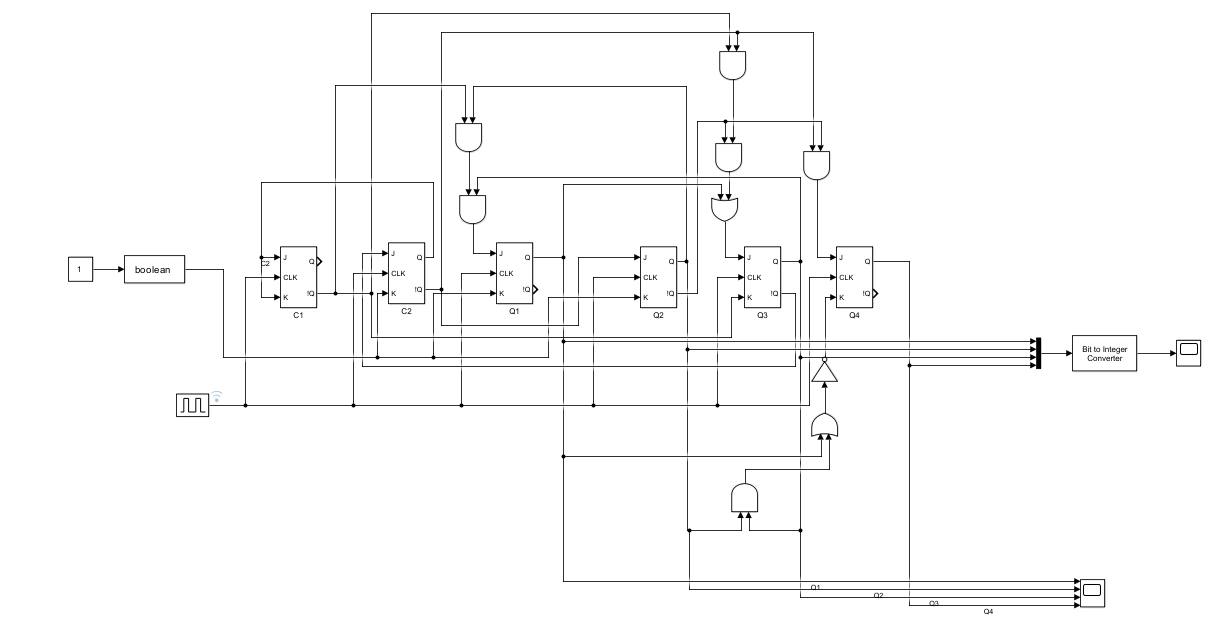
\includegraphics[width=\textwidth]{SImCircFinal.PNG}
    \caption{Simulated Circuit}
\end{figure}
\begin{figure}[!htb]
    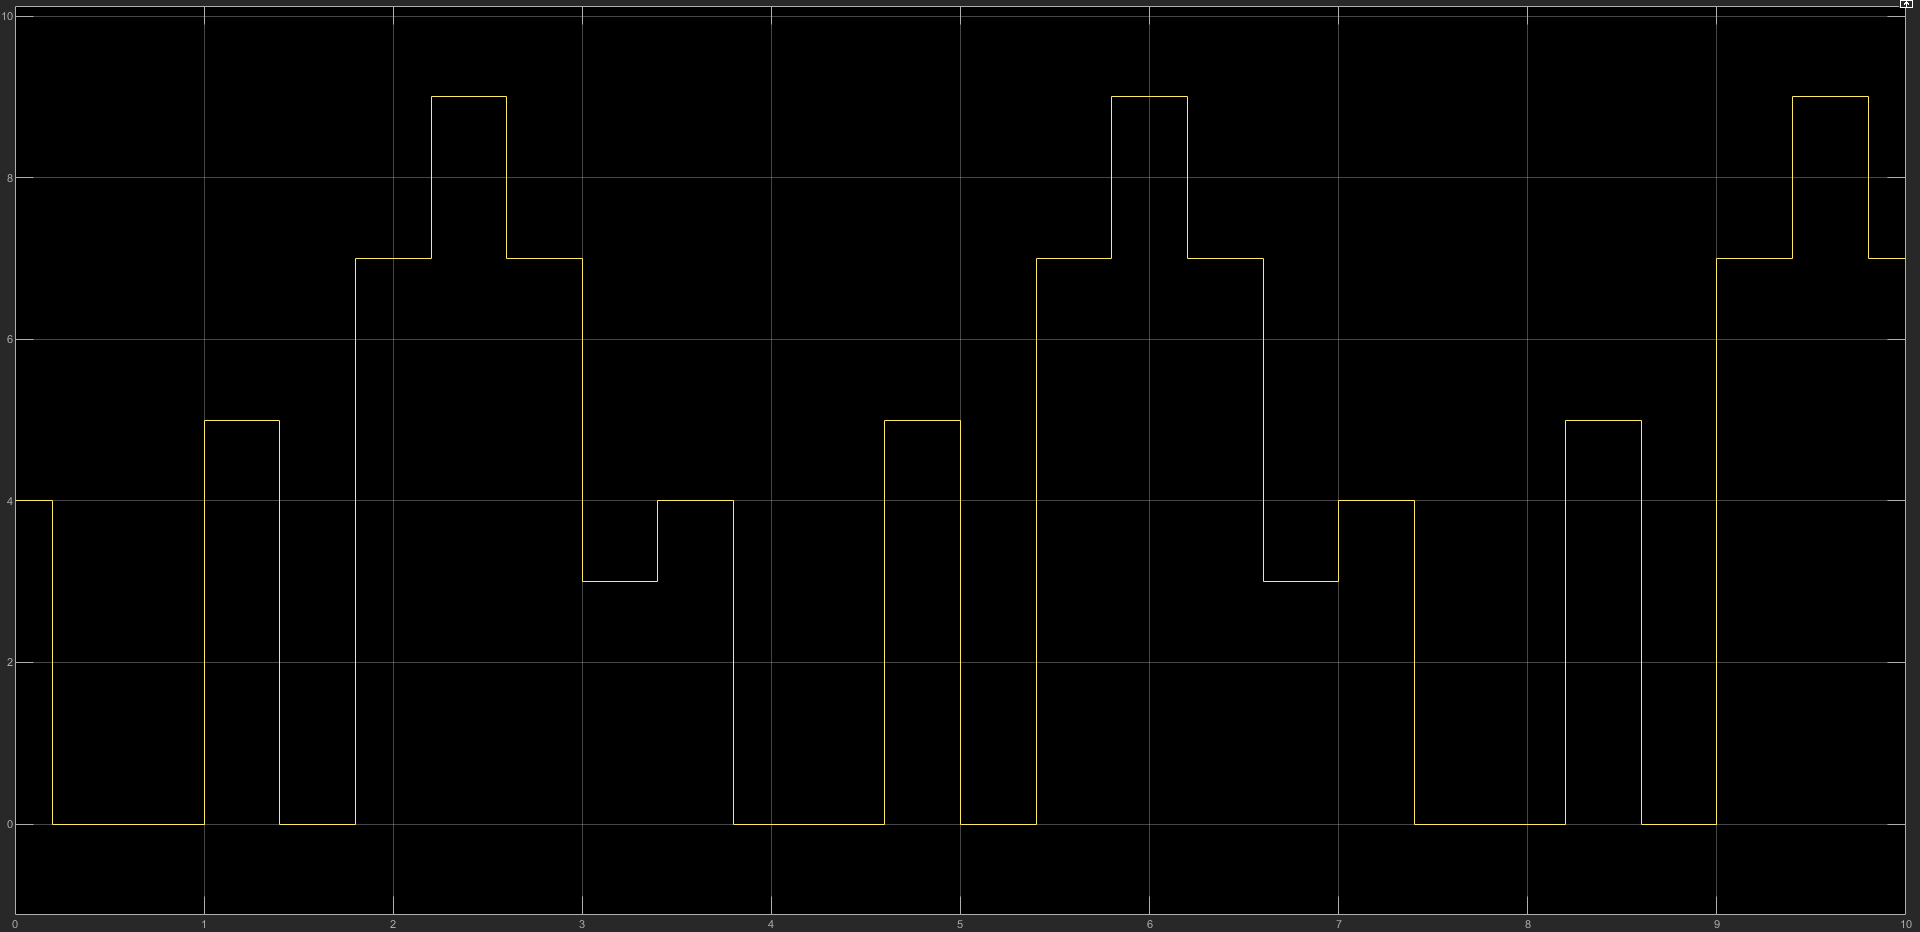
\includegraphics[width=\textwidth]{NumbersOutput.PNG}
    \caption{Binary To Integer Conversion of Qs}
    \label{fig:BitToIntQ}
\end{figure}
\begin{figure}[!htb]
    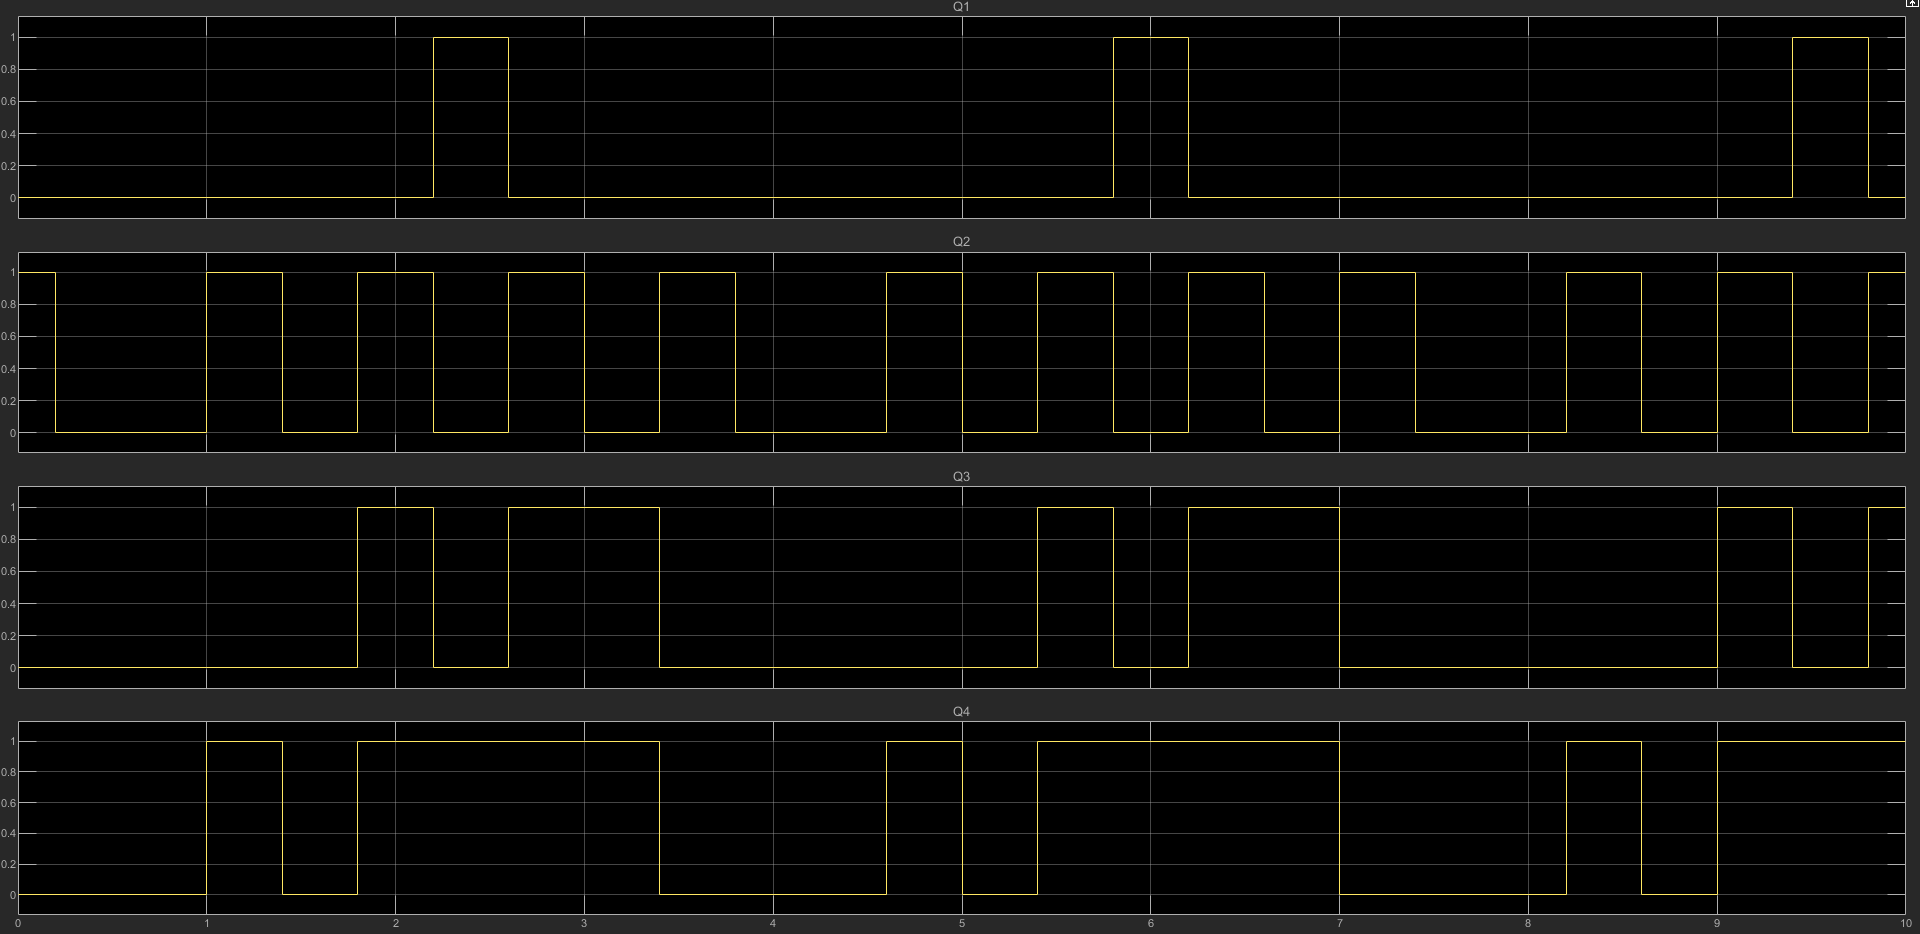
\includegraphics[width=\textwidth]{QTimings.PNG}
    \caption{Timing Diagrams of Q}
\end{figure}
\begin{figure}[!htb]
    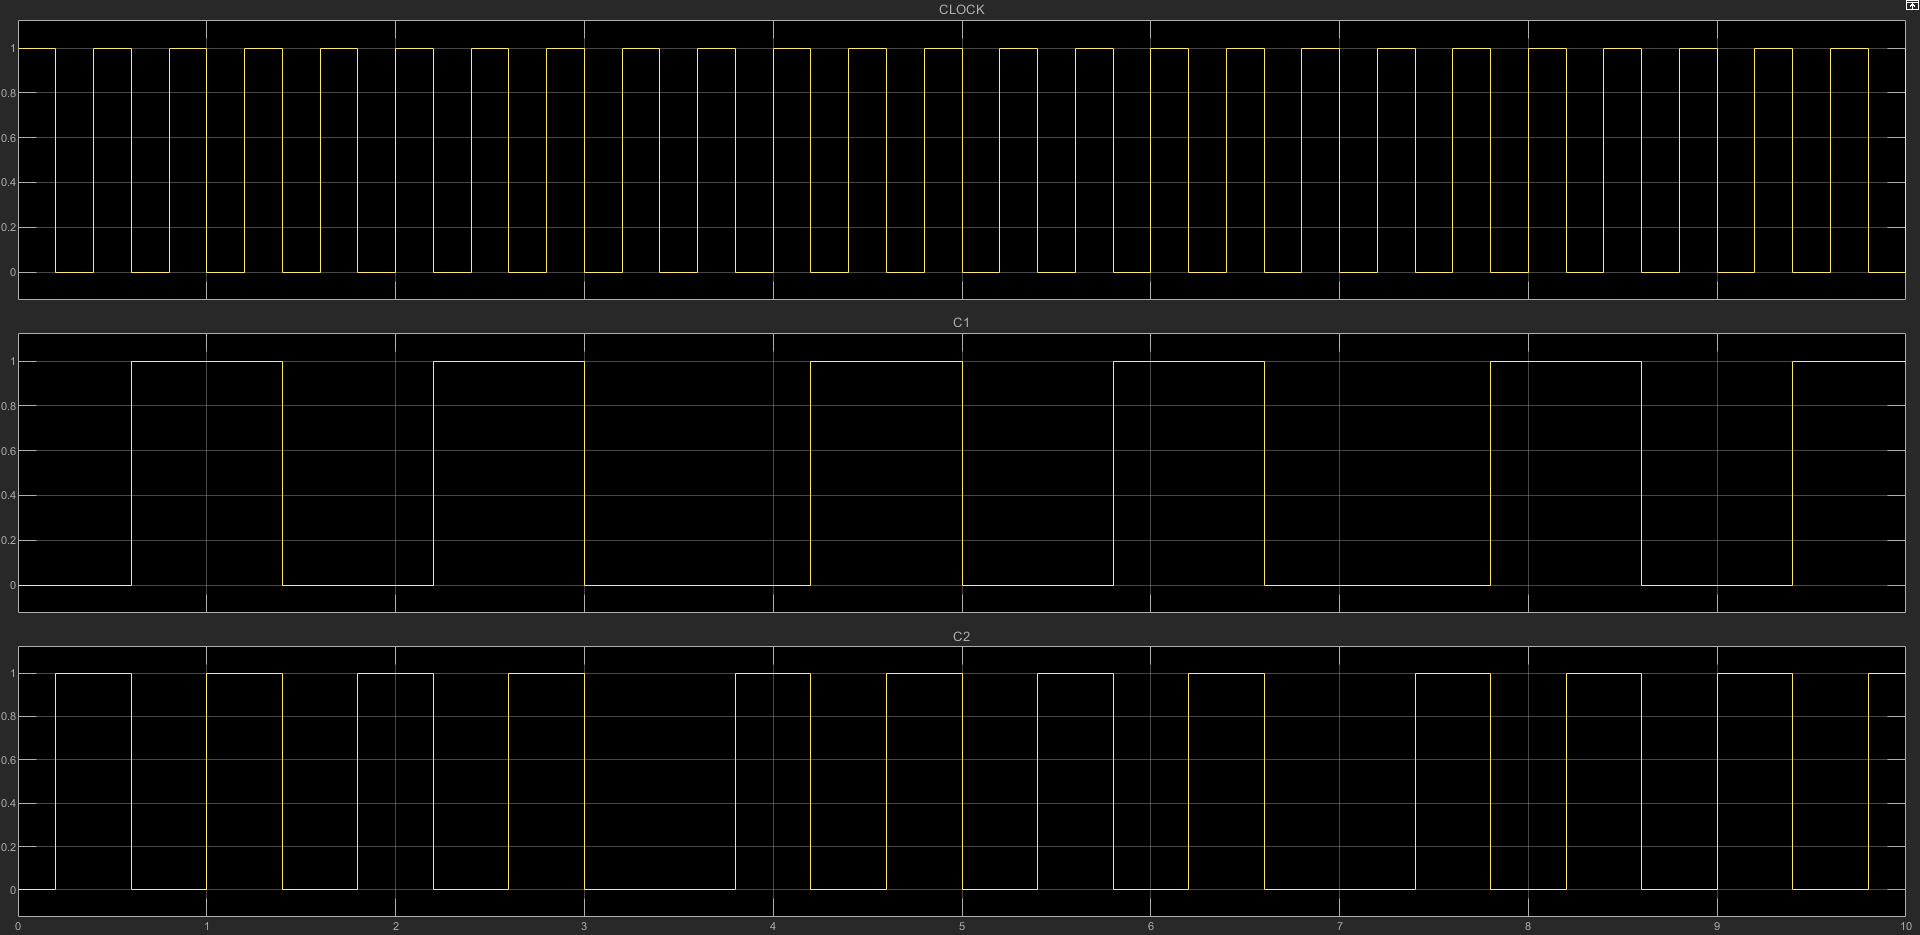
\includegraphics[width=\textwidth]{CandClockTimings.PNG}
    \caption{Timing Diagrams of C and Clock}
\end{figure}
\subsection{Discussion of Simulated Results}
We see that the all timings and output match expected results. The JK-Flip-Flops in Simulink however, are negative-edge triggered
thus will be out of phase by half a period, but otherwise will be unaffected. The output, shown in \hyperref[fig:BitToIntQ]{figure \ref{fig:BitToIntQ}}, shows the number student number 
400507973, being displayed sequentially at a clock frequency of 2.5Hz. As Simulink does not have a 7SD or 7SD encoder, a scope and bit/binary to integer converter was used 
in place of it, the physical build will include the ICs instead. While the Simulation's initial state is 000100, in the order of $C_1C_2Q_1Q_2Q_3Q_4$, for simplicity 
it can be started at 000000, as it is also a part of the stable loop, the third 0 in the student number.
\subsection{Debugging}
The circuit was initially:
\begin{figure}[!htb]
    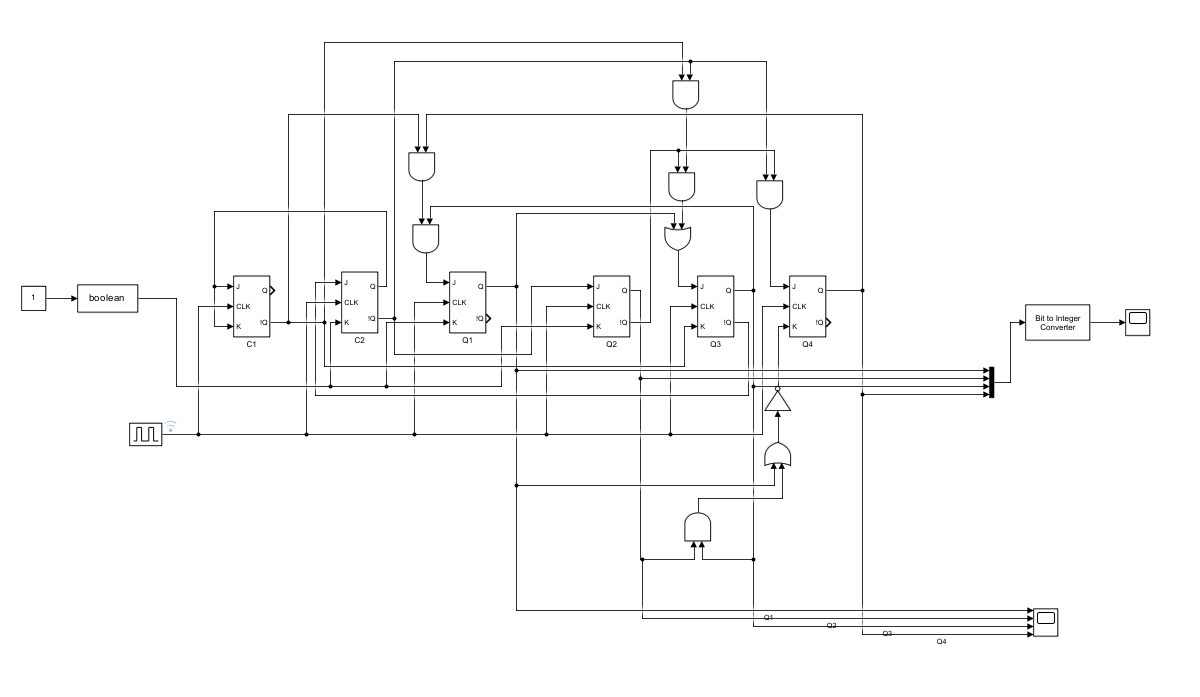
\includegraphics[width=\textwidth]{SimCircV1.PNG}
    \caption{Initial Implementation of Circuit in Simulation}
\end{figure}
\newpage
\begin{figure}[!htb]
    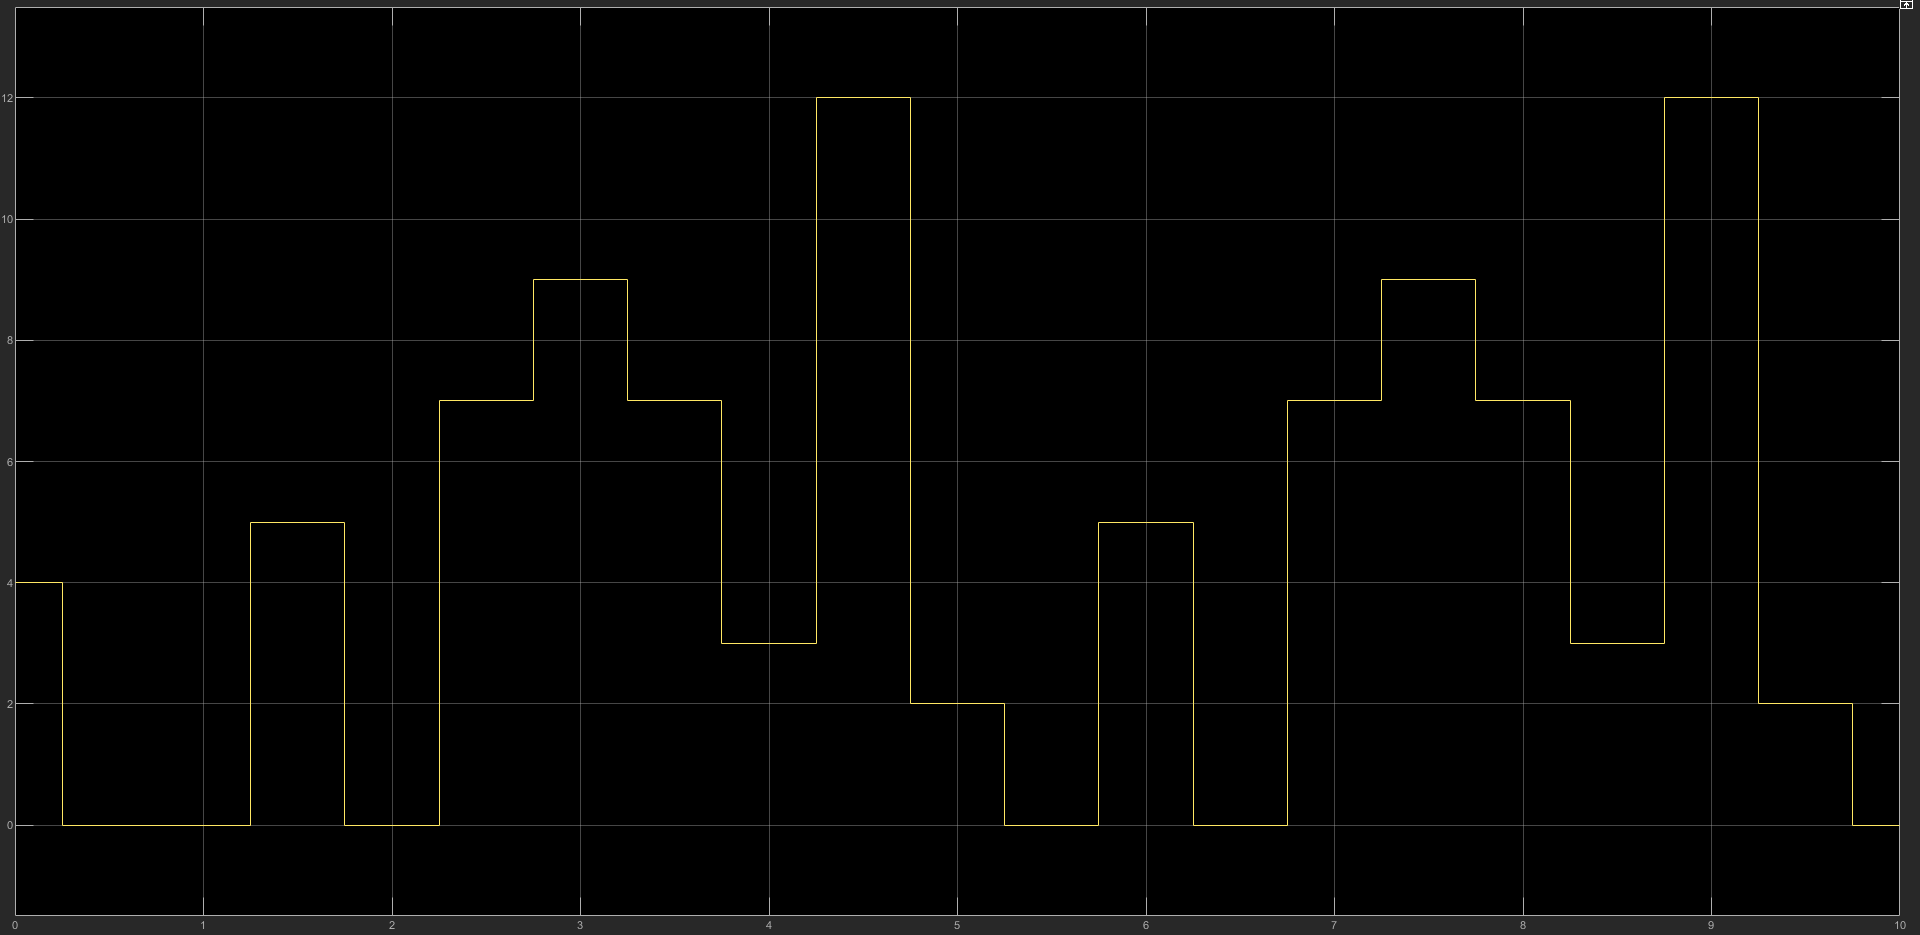
\includegraphics[width=\textwidth]{OutputV1.PNG}
    \caption{Initial Output of Circuit}
\end{figure}
From the above output, it can be observed that the initial loop correctly displays the student number. However, something goes wrong 
in following loops. The issue can be narrowed down by looking through the timing diagrams for each Q, and comparing these to the 
excitation table.
\begin{figure}[!htb]
    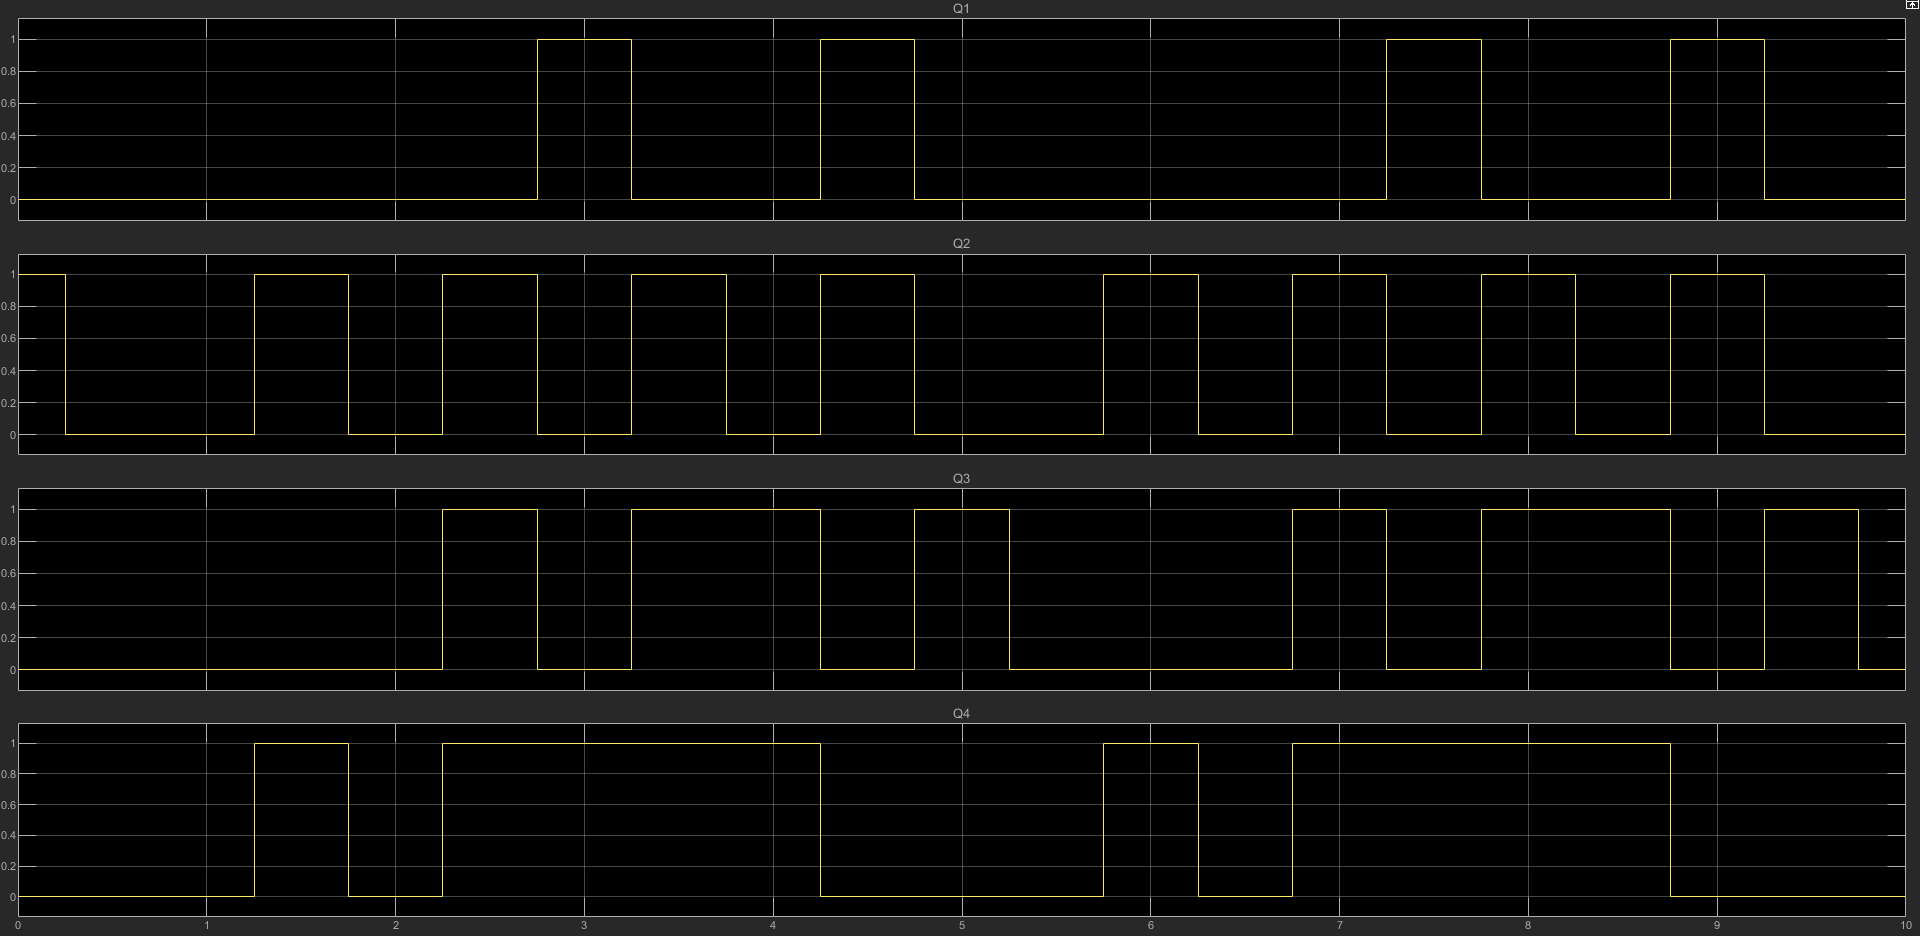
\includegraphics[width=\textwidth]{QsCheck.PNG}
    \caption{Scope for Output Qs}
\end{figure}
\\
From this graph we find that $Q_1$ becomes high an additional time. Reviewing the connections for $Q_1$, it was determined
that $Q_4$ was connected rather than $Q_2$. Changing this connection, we find the circuit to be working as intended, repeating all 
numbers in a cycle. Furthermore, as having a NOT gate would introduce a new IC 
\newpage
\section{Physical Circuit}
\end{document}